\documentclass{beamer}
\usepackage[utf8]{inputenc}
\usetheme{PaloAlto}
\usepackage{graphicx}

\title{AUTOMATIC RECONFIGURING NEWS SITE}
\begin{document}
\begin{frame}{}
\centering \textbf{ AUTOMATIC RECONFIGURING NEWS SITE} \newline \newline
\centering \textbf {           S5 CSB} \newline \newline
\centering\small Nikhill Shanmukhan \newline
\centering Sachit Anand \newline
\centering Siddharth Biju \newline
\centering Sidharth Sreekumar \newline
\end{frame}
	\begin{frame}{Page of Contents}
		\tableofcontents
	\end{frame}
	\section{Intro}
	\begin{frame}{Introduction}
	    
\includegraphics[width=10cm, height=5cm]{Shot.png}
		\begin{itemize}
			\item \Large{News is the information about an event happening right now.}
		\end{itemize}
	\end{frame}
	\begin{frame}{}
	    \begin{itemize}
			\item\Large Online news reading has become a popular way to read news articles from a huge collection of news sources all around.
			\item In this work we present a method for identifying top news in the web environment[1] that consists of diversified news portals. 
		\end{itemize}
	\end{frame}
	\section{Statement}
	\begin{frame}{Problem Statement}
	    \begin{itemize}
	        \item  \Large{News websites are one of the most visited destinations on the web.}
	        \item \Large { As there are many news portals created on a daily basis, each having its own preference for which news are important. Detecting unbiased[2] important and popular news are the problematic part of the news portal development.}
	    \end{itemize}
	\end{frame}
	\section{Approach}
	\begin{frame}{Approach 1}
		\begin{itemize}
			\item \Large \textbf{Hit Search Algorithm}
			  \newline Input: article dataset
			   \newline Output : Article order according to popularity
		\end{itemize}
		\Large{Step 1: Read dataset containing articles \newline
		Step 2: Extract title,Number of articles n \newline
		Step 3: Do steps 4,5 for n articles \newline
		Step 4: Search title using any search engine \newline
		Step 5: Read and store corresponding number of hits \newline
		Step 6: sort articles according to number of hits \newline
		Step 6: Do steps 7 for n articles \newline
		Step 7: Print title and content of sorted articles}
		
	\end{frame}
	\begin{frame}{Approach 2}
	\footnotesize
	\Large{Input: nil \\
	Output: website with popular news articles\\}
	\vspace{.2cm}
	\footnotesize
	\Large{step 1: For every 1 hour extract latest news article details from different\\ \hspace{1.2mm} news site 
	(includes TimeofPublish ,ups,downs)\\
	step 2:Find the number of articles extracted\\
	step 3: Using reddit hot ranking algorithm sort the news articles based on popularity rank\\
	step 4:Display each article based on the rank calculated.\\}
	\vspace{0.5cm}
	\end{frame}
	\begin{frame}{Approach 2 cont ...}
	\textbf{\Large{reddit hot ranking algorithm[4]:}}\\
	\Large{step 1:start\\
	step 2:for each article extract the time of publish,upcount,downcount\\
	step 3:set ep=1970,1,1 in datetime format\\
	step 4.define a function epsec(date)\\
	\hspace{.3cm}step 4.1:td=date - ep\\
	\hspace{.3cm}step 4.2:return td.days * 86400 + td.seconds +\\ \hspace{.8cm}(float(td.microseconds) / 1000000)\\
	step 5:define a function score(upcount,downcount)\\
	\hspace{.3cm}step 5.1:return upcount-downcount\\}
    \end{frame}
    \begin{frame}{Approach 2 cont ...}
    \Large{step 6:define a function hot(upcount,downcount,date)\\
    \hspace{.3cm}step 6.1:s = score(upcount, downcount)\\
    \hspace{.3cm}step 6.2:order = log(max(abs(s), 1), 10)\\
    \hspace{.3cm}step 6.3:sign = 1 if s is grater than 0 else -1 if s less than 0 else 0\\
    \hspace{.3cm}step 6.4:seconds = epsec(date) - 1134028003\\
    \hspace{.3cm}step 6.5:return round(sign * order + seconds / 45000, 7)\\
    step 7:stop}
    \end{frame}
	
	
	
	       
	
\begin{frame}{Approach 3}
		\footnotesize
	\Large{Input : nil \\
	Output :  website with trending news}
	
	\footnotesize
	\textbf{\Large{server side algorithm: }}\\
\Large{	step 1 :  for each 24 hours : \\
	\hspace{.2cm} step 1.1 : twurl /1.1/trends/place.json?id=1 > copy.json\\
	step 2:  data = file.read() \\
	step 3:  from i=0 to i=10 \\
	\hspace{.2cm}step 3.1: temp = data[0]["trends"][i]["name"]\\   
	\hspace{.2cm}Step 3.2:  temp = temp[1:]  \\
\hspace{.2cm}Step 3.3:  temp = temp + " latest news articles"\\
\hspace{.2cm}Step 3.4:  keyarray.append(temp)  \\
 }
		
	\end{frame}
	\begin{frame}{Approach 3 cont ...}
    \Large{	
    step 4: crawl google for news links using keyarray values\\
    step 5: seperate title and content from links obtained  and append to an array with id \\
    step 6: accept get request with news id\\
    step 7: return array[id]\\   }
    \\
    \\
	\footnotesize
	\textbf{\Large{client side algorithm: }}\\
	\Large{step 1 : render  navbar .js  \\	
	step 2:  render  contents .js \\}
\end{frame}
\begin{frame}{Approach 3 cont....}
    \Large{\vspace{5mm}
	\textbf{contents .js}\\
	\vspace{5mm}
	1. for(i=0;i<10;i++)\\
	\hspace{.2cm}1.1 get 127.0.0.1 with i as id\\
	\hspace{.2cm}1.2 store response in an array\\
	2. render title and contents in array}
    
\end{frame}
	\begin{frame}{Approach 4}
		   \begin{itemize}
        	\item \Large View Sort Algorithm\\
        	\footnotesize
        	\Large{Input: Nil\\
        	Output: Articles sorted based on popularity \\  }
   	   \end{itemize}	
           \Large{ Step 1:Search for all news sites with trending news using search engine\\
            Step 2:Repeat Step 3,4 until no more chances left\\
            Step 3:Views of every page is stored\\
            Step 4:Compare views of all pages\\
            Step 5:Content of page with high views is extracted\\
            }


	\end{frame}
	\begin{frame}{Approach 4 cont...}
	    \Large{
            Step 6:All articles extracted are sorted according to the number of views\\
            Step 7:Print title and content of sorted articles\\} 
        
            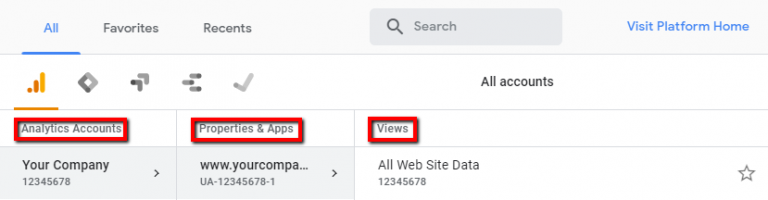
\includegraphics[scale=.38]{google.png}
	\end{frame}
	\section{Comparison}
	\begin{frame}{Comparison}
	\begin{itemize}
            \item \Large{On comparing Approach 1 and 4 ,Approach 1 takes only articles from twitter and articles may not be always available.      
            \item comparing Approach 4 and 2,Approach 2 its more difficult to implement to news articles as downvote[3] and upvote[4] my not be present in all articles.}
  	    \end{itemize}
  	 \end{frame}
    \begin{frame}{Comparison contd..}
        \begin{itemize}
            \item \Large {Approach 3 has  possible cases of HTTP error and popularity may not be accurate}
        \end{itemize}
	\end{frame}
	\section{Solution and Conclusion}
	
	\begin{frame}{Solution and Conclusion}
	\begin{itemize}
	
	\item \Large In this work, we propose a method to detect and to rank important news stories in web environment
	\item \Largeuse  We use google search to fetch news from all website.
	\item \Largeuse  Then we analyze the total views of all website using google analytics.
	\item \Largeuse  After that we separate the title and content of the news articles and display it.
	\end{itemize}
	\end{frame}
	\section{Ethical and Social Relevance}
	\begin{frame}{Relevance}
	\begin{itemize}
	    \item \Large{Our websites gives the latest and popular information to the public – political, social, sports, entertainment etc.}
	    \item \Large {The site play a vital role in educating and informing Mass with latest updates, current happenings around the globe.}
	\end{itemize}
	\end{frame}

	
	\section{Reference}
	\begin{frame}{Reference}
	    [1]https://www.ibm.com/
	    \newline\newline
	    [2]https://en.wikipedia.org/
	    \newline\newline
	    [3]https://en.wiktionary.org/
	    \newline \newline
	    [4]https://medium.com/hacking-and-gonzo/how-reddit-ranking-algorithms-work-ef111e33d0d9
	     \end{frame}
\end{document}